\documentclass[11pt, twoside, a4paper]{report}

\usepackage{verbatim}
\usepackage{tikz}
\usetikzlibrary{arrows,shapes}
\tikzstyle{vertex} = [circle, fill=black!25, minimum size=100pt, inner sep=0pt]
\tikzstyle{edge} = [draw, thick, line width=1.5pt, inner sep=5pt, outer sep=5pt]

\begin{document}

\title{Perceiving and memorising packaged goods \\ (in a supermarket environment)}
\author{Carsten K\"onemann \\ \texttt{cargath@gmail.com}}
\date{08.10.2013}

\maketitle

% \chapter{Abstract}

% Wohin Debugging / Testing ?

\tableofcontents

\chapter{Introduction}

\section{Review}

\section{Motivation}

\section{Goal}

\section{Structure}


\chapter{Scenario}


\chapter{Methods}

\section{}
\subsection{ROS}
\subsection{OpenCV}
\subsection{SiftGPU}

\section{Architecture} % Oder UML? Oder ist das zu Implementationsspezifisch?

\begin{figure}
  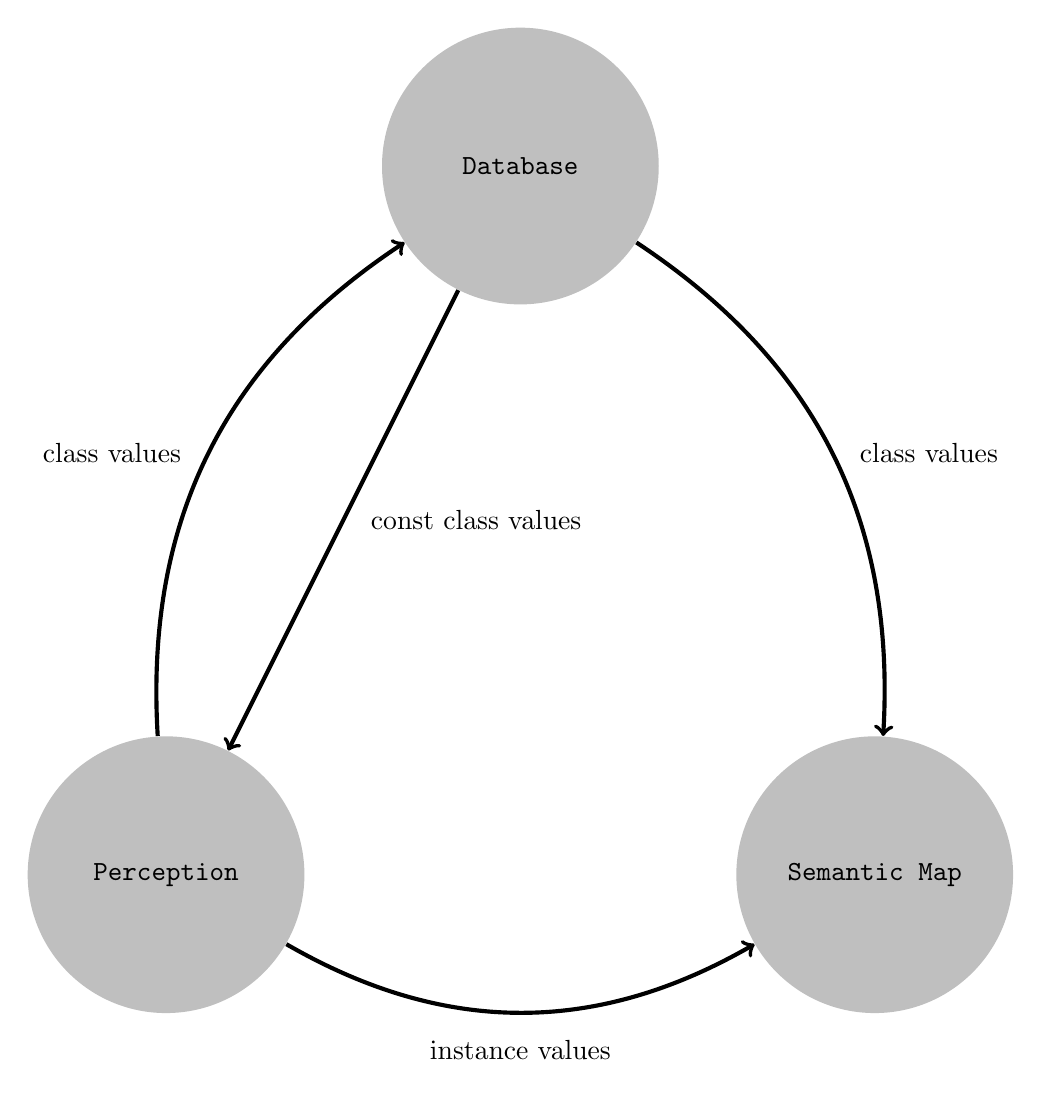
\begin{tikzpicture}[->, scale=1.8, auto, swap]
    % Draw the vertices.
    \node [vertex] (a) at (2.5, 5) {\texttt{Database}};
    \node [vertex] (b) at (  0, 0) {\texttt{Perception}};
    \node [vertex] (c) at (  5, 0) {\texttt{Semantic Map}};
    % Database <-> Perception.
    \path [edge] (a) edge [] node [right] {const class values} (b);
    \path [edge] (b) edge [bend left] node [left] {class values} (a);
    % Perception -> Semantic Map.
    \path [edge] (b) edge [bend right] node {instance values} (c);
    % Database -> Semantic Map.
    \path [edge] (a) edge [bend left] node [right] {class values} (c);
  \end{tikzpicture}
\end{figure}

\subsection{Database}
\subsection{Perception}
\subsection{Semantic Map}

\section{Implementation}
\subsection{Shared Library}
\subsection{Setup Samples}
\subsection{Mipmapping}
\subsection{Feature Detection and Matching}
\subsection{Filter Matches}
\subsection{Filter False Positives}
\subsection{Calculate 3D Pose}
\subsection{Memorise only new Objects}
\subsection{Evaluation Function}


\chapter{Results}


\chapter{Discussion}


\chapter{Conclusion}


\end{document}
